\section{Nombre: Etalagmitas}\label{obs.rocas}
	\subsection{Descripción}
	Tres estalagmitas de tamaño mediano, se ubican sobre el techo de cuevas. Cuando el jugador pasa por debajo de ellas caen. Al hacer contacto con el jugador le reducen la cantidad de vida.
	\subsection{Esquema}
Ver figura \ref{fig:estalagmitas}.
	\begin{figure}
  \centering
  \subfigure[El jugador se aproxima a la zona de las estalagmitas.]{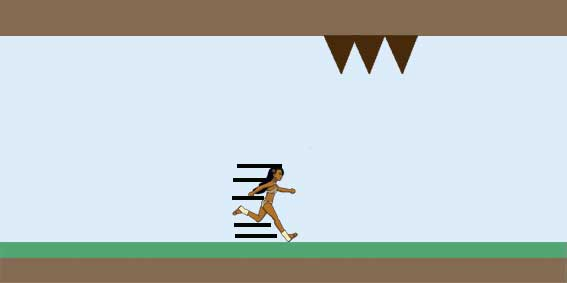
\includegraphics[width=0.3 \textwidth]{Imagenes/estalagmitas01}}
   \subfigure[Cuando el jugador se posiciona bajo las estalagmitas, las estalagmitas caen.]{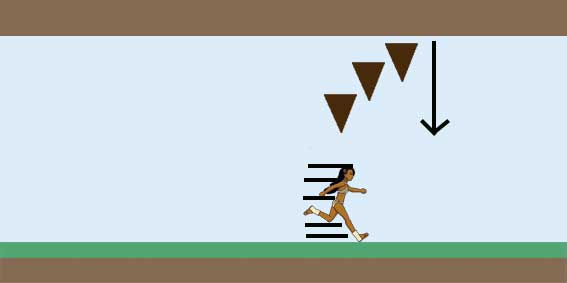
\includegraphics[width=0.3 \textwidth]{Imagenes/estalagmitas02}}
  \caption{Plataforma que cae.}
  \label{fig:estalagmitas}
\end{figure} 